\section{Inertial Measurement Unit (IMU)}
An inertial measurement unit (IMU) is an electronic device that measures linear and angular motion, usually with the combination of accelerometers and gyroscopes, but sometimes also with magnetometers. As described in \cref{chap:myo}, the Myo armband provide data from accelerometer, gyroscope and magnetometer. These are three sensors useful to determine position and orientation, but they measure different things.

\subsection{Gyroscope}
The gyroscope is used to measure or maintain the angular position. It consist of a disc (the rotor) that spins about an axis. Based on the principle of conservation of angular momentum, a spinning rotor will maintain it's orientation, thus the axis will be unaffected by tilts or rotations \cite{gyroscope_demonstration_project}. We can separate gyroscopes into three basic types:

\begin{itemize}
    \item Rotary (classical) Gyroscopes
    \item Vibrating Structure Gyroscopes
    \item Optical Gyroscopes
\end{itemize}

The gyroscope measure the angular velocity of the rotor. Since vibrating structure gyroscopes with MEMS technology are widely used in smart-phones and other electronic devices, we will take a closer look at vibrating structure gyroscopes \cite{vibrating_structure_gyroscope_wiki}. To better understand vibrating structure gyroscopes we need a basic understanding of the Coriolis effect. Every point on a rotating system will have the same angular velocity, but in order to travel a straight line towards or away from the axis of rotation, the traveling object have to either increase or decrease the linear velocity in order to maintain the relative angular position. The acceleration required to maintain the relative angular position is the Coriolis acceleration, an example is shown in \cref{fig:coriolis_acceleration} \cite{vibrating_structure_gyroscope}. Vibrating object tends to continue vibrating in the same plane even if its support rotates. The Coriolis effect causes the object to apply a force on its support, and by measuring this force the angular velocity can be determined \cite{vibrating_structure_gyroscope_wiki}.

\begin{figure}[ht]
    \centering
    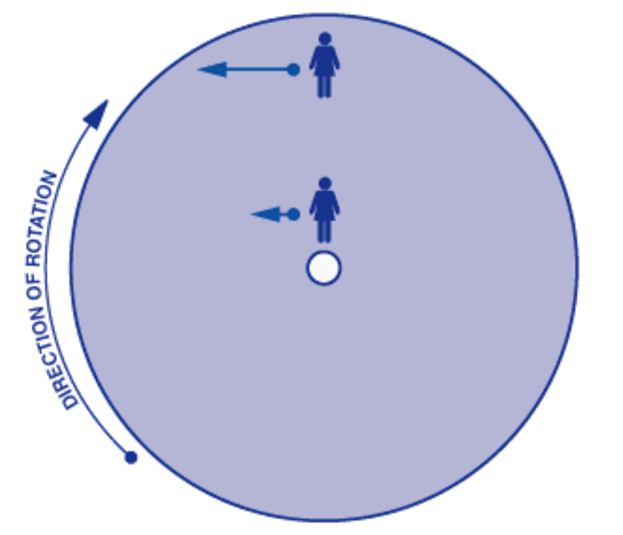
\includegraphics[height=5cm]{images/coriolis_acceleration.jpg}
    \captionsource{\url{http://www.analog.com/en/analog-dialogue/articles/imems-angular-rate-sensing-gyroscope.html}}
    \caption[Coriolis Acceleration Example]{A person trying to move northward toward the outer edge of a rotating platform. The linear velocity (Blue linear arrows) has to increase in order to maintain a northbound course. The acceleration is the Coriolis acceleration.}
    \label{fig:coriolis_acceleration}
\end{figure}


\subsection{Accelerometer}
An accelerometer is an electromechanical device to measure proper acceleration. Proper acceleration should not be confused with coordinate acceleration (rate of change of velocity). The measurement unit is given by g-forces ($g \approx 9.81m/s^{2}$), and by contrast to measuring coordinate acceleration, accelerometers in free fall will measure zero. 

There are many type of accelerometers, but to understand how the accelerometer work, we can use a simple model. Have in mind that this model is not exactly how a MEMS sensor work, but it explains the basic concept of accelerometers. To make this model simple, we will use a representation as shown in \cref{fig:accelerometer_model}. Imagine a ball inside a cube, when gravity pulls the ball down, it will hit at least one of the walls. The wall will according to Newton's third law have a force against the ball. This force is the measurement the accelerometer returns. This value can be represented by a vector \cite{IMU_guide}.

\begin{figure}[ht]
    \centering
    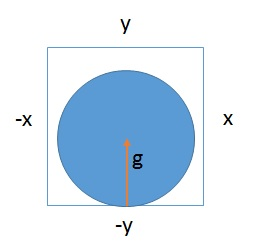
\includegraphics[height=5cm]{images/accelerometer.jpg}
    \caption[Accelerometer model]{2D representation model of a simple concept of an accelerometer. A ball is pushed down by gravity, and the accelerometer measure 1g at the -y wall.}
    \label{fig:accelerometer_model}
\end{figure}

\subsection{Magnetometer}
Orientation of a static or slow-moving rigid body can be determined from the measured gravity and local magnetic field vectors \cite{yun2008simplified}. Magnetometer is a device that measure magnetic fields, either the magnetization of magnetic materials, or the strength and the direction of the magnetic field at a point in space \cite{magnetometer_wiki}. The magnetometer from the Myo armband returns the orientation as unit quaternion \cite{myoSDK}. Quaternions provide a mathematical notation for representing orientation and rotation in the three dimensional space. Quaternions is described in more detail in \cref{sec:quaternion}.
 
